%!TEX root = Slic3r-Manual.tex

\subsection{Multiple Extruders} % (fold)
\label{sec:multiple_extruders}
\index{extruders!multiple}

A printer with more than one extruder can be used in different ways: The additional extruder could print a different color or material; or it could be assigned to print particular features, such as infill, support or perimeters.

Multi-material printing requires a suitably designed object usually written in AMF format as this can handle multiple materials (see Model Formats in §\ref{sub:model_formats}).  Details on how to create such a file are given below.


\subsubsection{Configuring Extruders} % (fold)
\label{sub:configuring_extruders}
\index{Printer Settings!General!Capabilities!Extruders}

In the \texttt{Printer Settings} tab there is an \texttt{Extruders} option, under \texttt{Capabilities}, which allows the number of extruders to be defined.  Incrementing this value will dynamically add another extruder definition to the left-hand pane.

\begin{figure}[H]
\centering
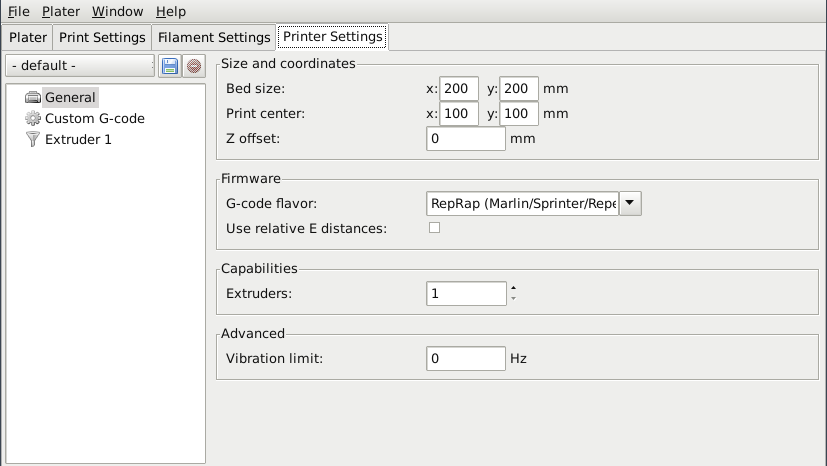
\includegraphics[keepaspectratio=true,width=1\textwidth]{expertmode/multipleextruders/printer_settings_general_multiple_extruder_options.png}
\caption{Multiple extruder options - Printer Settings Tab (General).  Note the two extruders defined in the left-hand pane.}
\label{fig:printer_settings_general_multiple_extruder_options}
\end{figure}

Each extruder can be configured as usual, however there are additional settings which must be set which are particular to multi-extruder setups.

\begin{figure}[H]
\centering
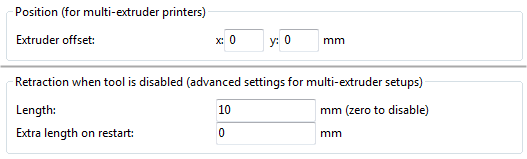
\includegraphics[keepaspectratio=true,width=1\textwidth]{expertmode/multipleextruders/printer_settings_extruder_multiple_extruder_options.png}
\caption{Multiple extruder options - Printer Settings Tab (Extruder).}
\label{fig:printer_settings_extruder_multiple_extruder_options}
\end{figure}

\index{Printer Settings!Extruder!Extruder offset}

The \texttt{Extruder offset} is to be used should the firmware not handle the displacement of each additional nozzle.  Your firmware documentation should tell you if this is the case.  Each additional extruder is given an offset in relation to the first one.  If the firmware does handle this then all offsets can remain at 0,0.

\index{Printer Settings!Extruder!Retraction!Length}
Because the secondary extruder will be dormant whilst the first is working, and vice-versa, it is important that the material is sufficiently retracted to stop oozing.  As with the regular retraction settings (see p.\pageref{fig:retraction_settings}) the \texttt{Length} options is measured from the raw filament entering the extruder.

% subsubsection configuring_extruders (end)

\subsubsection{Assigning Filaments} % (fold)
\label{sub:assigning_filaments}
\index{Plater}
When a printer profile with multiple extruders has been selected the \texttt{Plater} tab allows the selection of a different filament for each extruder.

\begin{figure}[H]
\centering
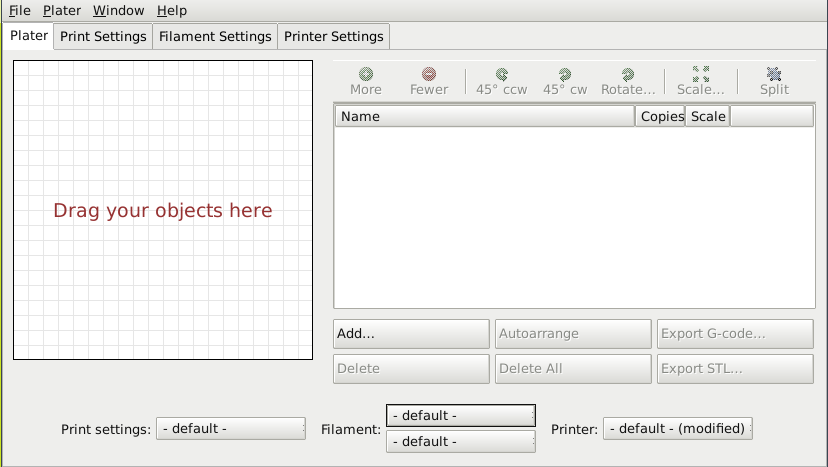
\includegraphics[keepaspectratio=true,width=1\textwidth]{expertmode/multipleextruders/plater_multi_filament.png}
\caption{Plater with multiple filament options.}
\label{fig:plater_multi_filament}
\end{figure}

% subsubsection assigning_filaments (end)

\subsubsection{Assigning Extruders for Single-material Objects} % (fold)
\label{sub:assigning_extruders}
\index{Print Settings!Multiple Extruders}

For single material prints, where the secondary extruder is to be tasked with a particular extrusion, the \texttt{Multiple Extruders} subsection of the \texttt{Print Settings} tab gives the ability to assign an extruder to each extrusion type.

\begin{figure}[H]
\centering
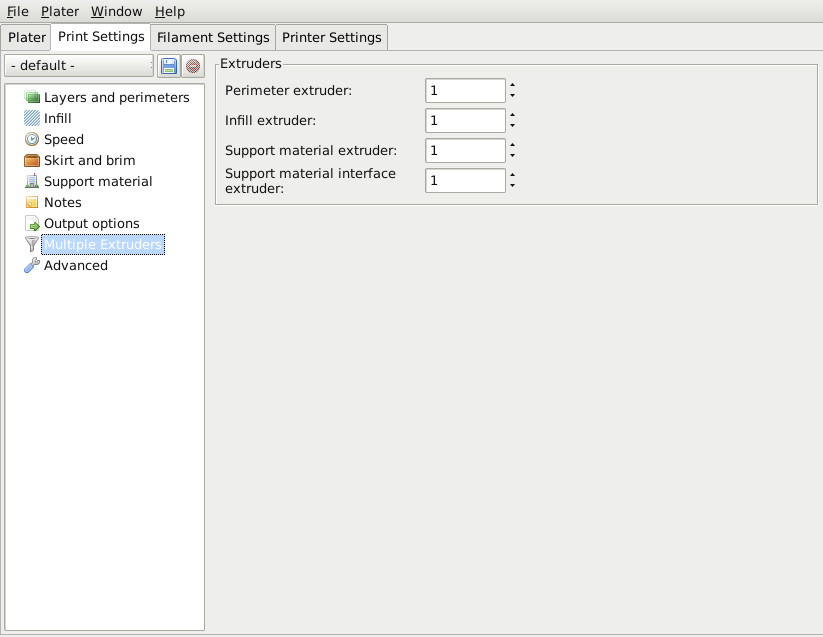
\includegraphics[keepaspectratio=true,width=1\textwidth]{expertmode/multipleextruders/print_settings_multiple_extruder_options.png}
\caption{Multiple extruder options - Print Settings Tab.}
\label{fig:advanced_multiple_extruder_options}
\end{figure}

% subsubsection assigning_extruders (end)

\subsubsection{Configuring Tool Changes} % (fold)
\label{sub:configuring_tool_changes}

\index{Printer Settings!Custom G-code!Tool change G-code}

The \texttt{Custom G-code} subsection of the \texttt{Printer Settings} tab has an option for inserting G-code between tool changes.  As with all custom G-code subsections, placeholder variables can be used to reference Slic3r settings.  This includes the [previous\_extruder] and [next\_extruder] variables.

\begin{figure}[H]
\centering
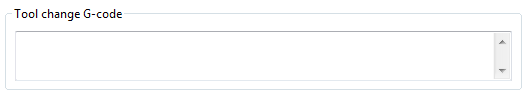
\includegraphics[keepaspectratio=true,width=1\textwidth]{expertmode/multipleextruders/printer_settings_custom_gcode.png}
\caption{Multiple extruder options - Tool change G-code.}
\label{fig:printer_settings_custom_gcode}
\end{figure}

% subsubsection configuring_tool_changes (end)


\subsubsection{Printing Multi-material Objects} % (fold)
\label{sub:printing_multi_material_objects}

If a multi-material AMF file already exists, because the CAD program can export such a format, then this can be loaded into Slic3r in the usual way.  The mapping between object materials and extruders is sequential, i.e. the first material is assigned to the first extruder, etc.

% subsubsection printing_multi_material_objects (end)


\subsubsection{Generating multi-material AMF files} % (fold)
\label{sub:generating_multi_material_amf_files}

Slic3r has the feature to combine multiple STL files into a multi-material AMF file.

\index{Menu!Combine multi-material STL files...}

\begin{itemize}
    \item Split the original design into the separate parts within the CAD program, and export each part as STL.
    \item Within Slic3r, choose \texttt{Combine multi-material STL files...} from the \texttt{File} menu.
    \item When prompted with a file dialog, choose the first STL, which will be assigned the first material (and hence the first extruder). Click \texttt{Open} to be prompted for the next STL, and so on until each STL is assigned a material.  To signal there are no more STL files, choose \texttt{Cancel}.
    \item The following file dialog prompts for the location and name of the AMF file.
\end{itemize}

Once generated the file can be loaded and printed as described above.

% subsubsection generating_multi_material_amf_files (end)

% subsection multipe_extruders (end)
